\section{Resultados e Discuss�es sobre a Sequ�ncia de Aplica��o}\label{sec:an�lise_sequ�ncia}

Esta se��o constar� a an�lise dos resultados obtidos durante a sequ�ncia did�tica de aplica��o.

\subsection{An�lise da Pesquisa Inicial}\label{subsec:an�lise_aula_1}

\begin{grafico}[ht]
	\centering
	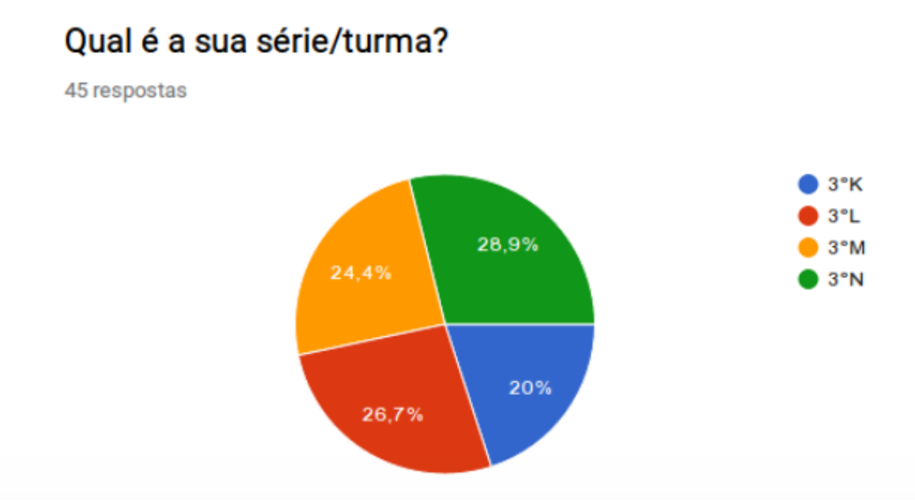
\includegraphics[width=0.8 \textwidth]{Resultados_e_Discussoes/Img_pesq_ini/resp_pesq_ini_01}
	\caption{Pesquisa Inicial: Introdu��o}
	\label{fig:rd_int}
\end{grafico}

\begin{grafico}[ht]
	\centering
	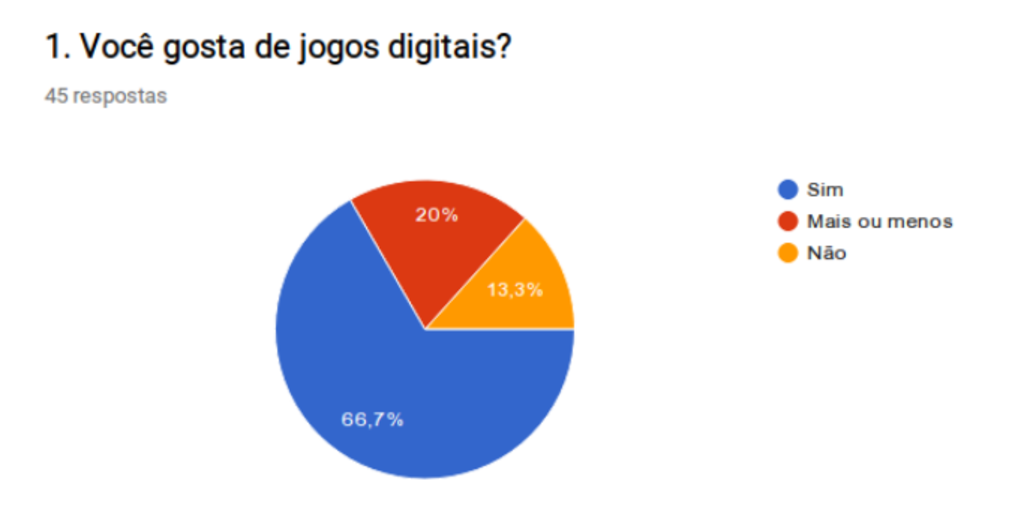
\includegraphics[width=0.9 \textwidth]{Resultados_e_Discussoes/Img_pesq_ini/resp_pesq_ini_02}
	\caption{Resultado: pergunta 1}
	\label{fig:rd_perg1}
\end{grafico}

\begin{grafico}[ht]
	\centering
	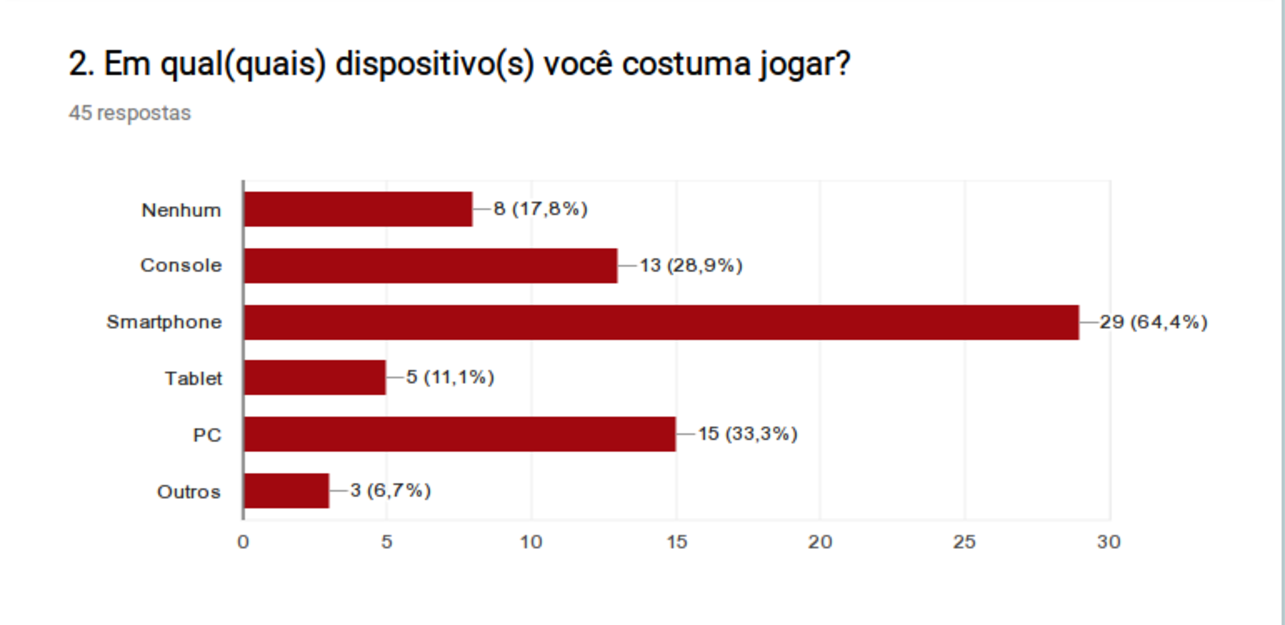
\includegraphics[width=1.1 \textwidth]{Resultados_e_Discussoes/Img_pesq_ini/resp_pesq_ini_03}
	\caption{Resultado: pergunta 2}
	\label{fig:rd_perg2}
\end{grafico}

\begin{grafico}[ht]
	\centering
	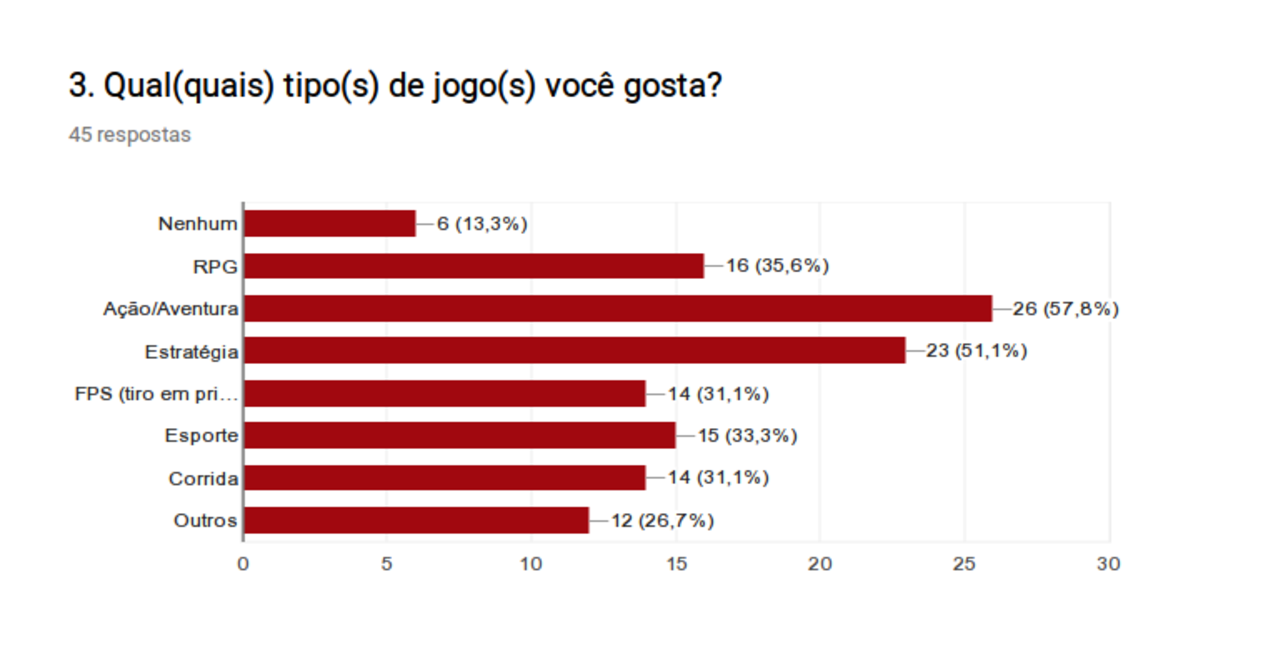
\includegraphics[width=1.1 \textwidth]{Resultados_e_Discussoes/Img_pesq_ini/resp_pesq_ini_04}
	\caption{Resultado: pergunta 3}
	\label{fig:rd_perg3}
\end{grafico}

\begin{grafico}[ht]
	\centering
	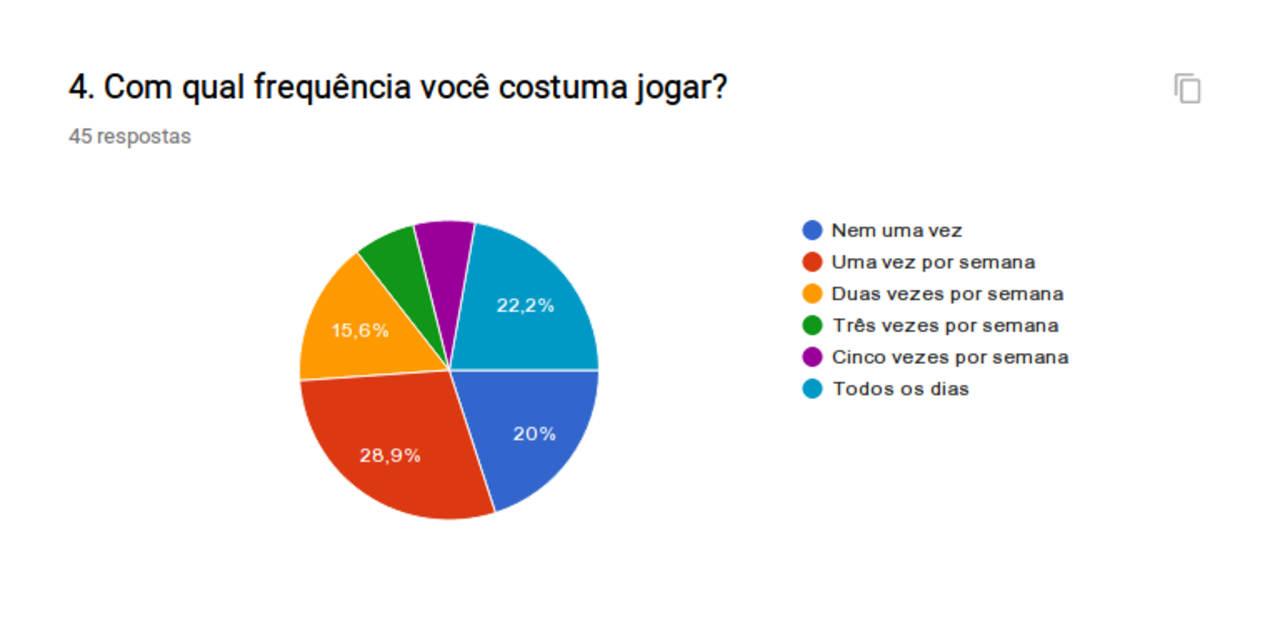
\includegraphics[width=1.1 \textwidth]{Resultados_e_Discussoes/Img_pesq_ini/resp_pesq_ini_05}
	\caption{Resultado: pergunta 4}
	\label{fig:rd_perg4}
\end{grafico}

\begin{grafico}[ht]
	\centering
	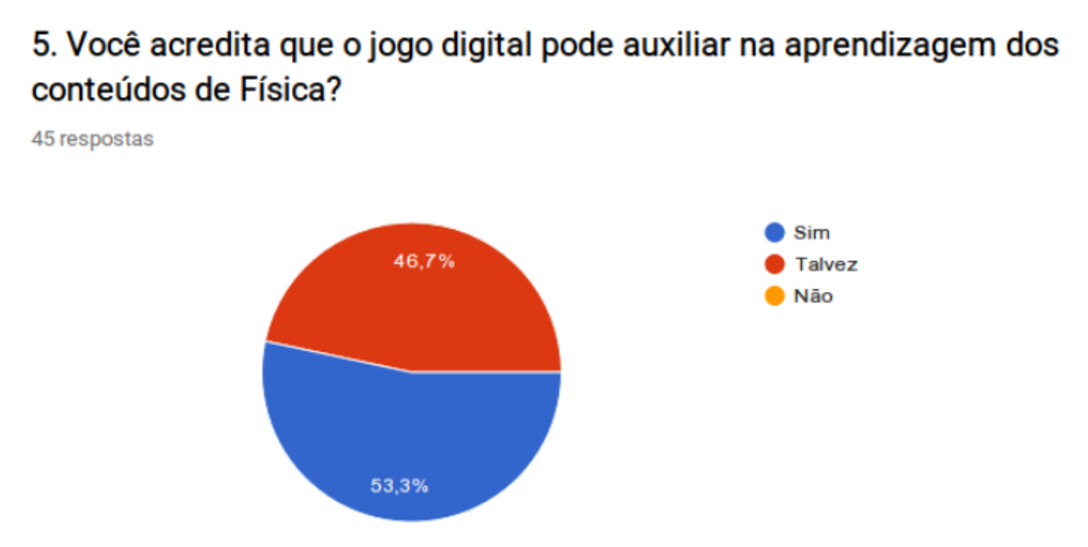
\includegraphics[width=0.9 \textwidth]{Resultados_e_Discussoes/Img_pesq_ini/resp_pesq_ini_06}
	\caption{Resultado: pergunta 5}
	\label{fig:rd_perg5}
\end{grafico}


\subsection{An�lise do Pr�-Teste}\label{subsec:an�lise_aula_2}

\begin{grafico}[ht]
	\centering
	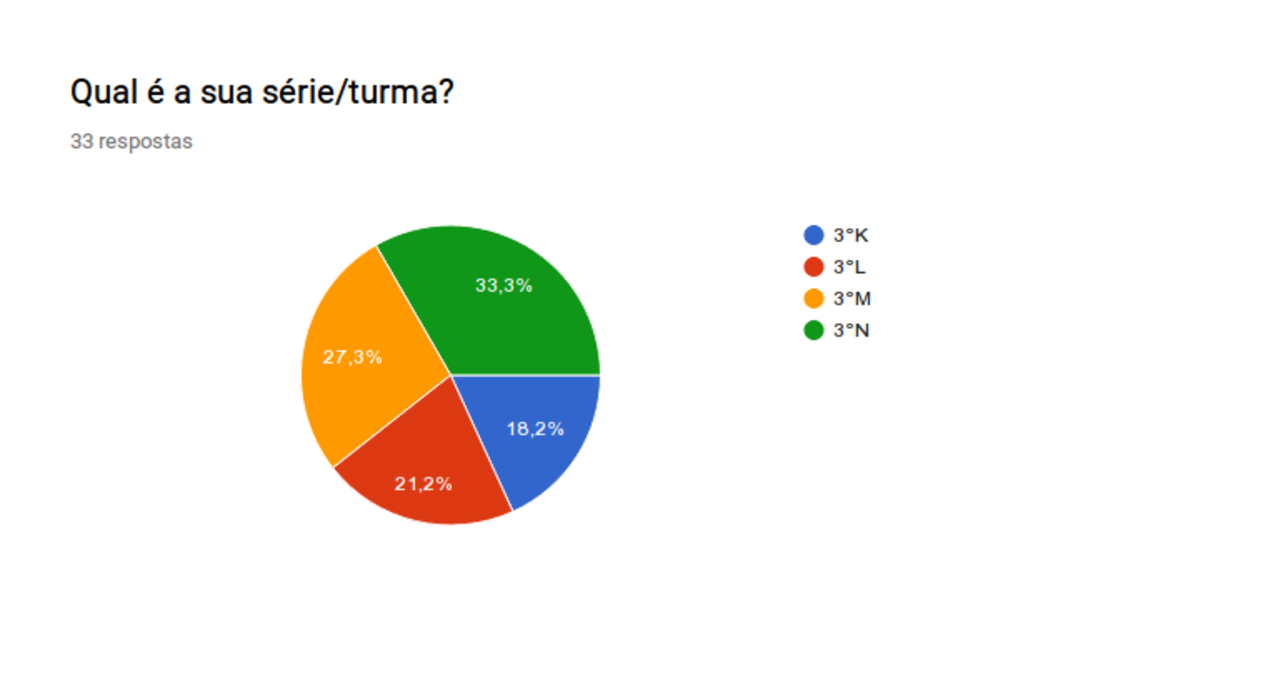
\includegraphics[width=1.1 \textwidth]{Resultados_e_Discussoes/Img_pre_teste/resp_pre_teste_01}
	\caption{Introdu��o}
	\label{fig:rd_perg5}
\end{grafico}

\begin{grafico}[ht]
	\centering
	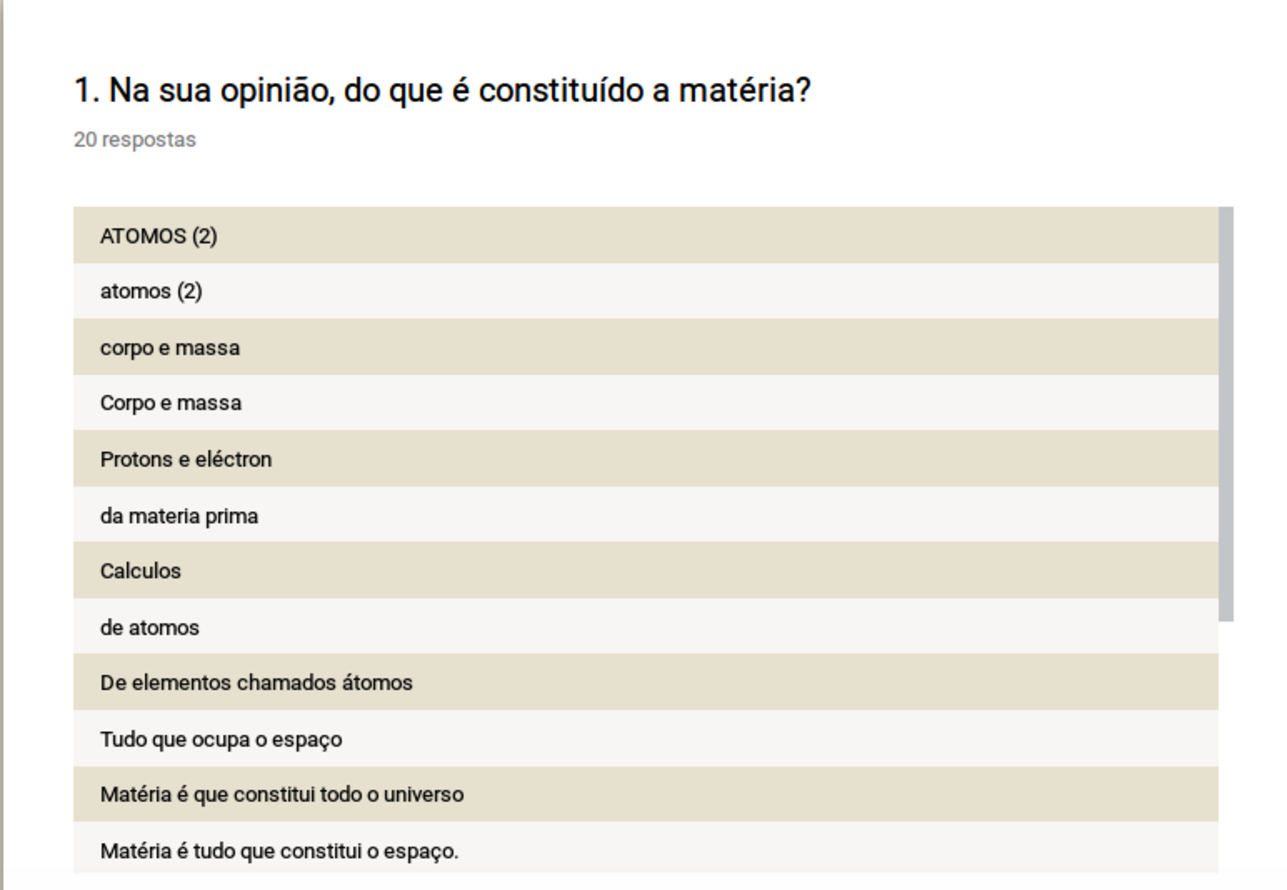
\includegraphics[width=1.1 \textwidth]{Resultados_e_Discussoes/Img_pre_teste/resp_pre_teste_02}
	\caption{Introdu��o}
	\label{fig:rd_perg5}
\end{grafico}


\subsection{An�lise da Primeira Aplica��o do Jogo}\label{subsec:an�lise_aula_3}
\subsection{Discuss�es sobre o V�deo: \aspas{O Discreto Charme das Part�culas Elementares}}\label{subsec:an�lise_aula_4_5}
\subsection{An�lise das Aulas Expositivas 1 e 2}\label{subsec:an�lise_aula_6_7}
\subsection{An�lise da Segunda Aplica��o do Jogo}\label{subsec:an�lise_aula_8}
\subsection{An�lise do P�s-Teste}\label{subsec:an�lise_aula_9}
\subsection{An�lise da Pesquisa Final}\label{subsec:an�lise_aula_10}

Aqui farei um compara��o entre o resultado esperado e o obtido, tendo como base os marcos te�ricos.